\chapter{Modellazione delle serie finanziarie e costruzione del grafo}
\label{ch:financial-series-and-graph-construction}

\section{Serie storiche finanziarie: rendimenti e loro proprietà}
\label{sec:financial-time-series-returns}

I \Cref{ch:mathematical-foundations,ch:from-cnn-to-gnn} hanno costruito, rispettivamente, la matematica dei grafi e l'architettura che apprende su tale struttura, assumendo dati già disponibili sotto forma di segnale sui nodi e di matrice dei pesi. Questo capitolo colma la distanza tra quest'assunzione e i dati reali, riprendendo tre punti lasciati in sospeso: il segno dei pesi (\cref{rem:negative-weights}), la densità del grafo (\cref{sec:known-limitations-gnn}) e la legittimità stessa della correlazione come peso (\cref{sec:message-passing-paradigm}).

\subsection{Dai prezzi ai rendimenti}

Il dato grezzo è la serie dei prezzi $P_t$ di un asset. Non si tratta tuttavia della quantità su cui si modella, per due ragioni. La prima è di scala: una variazione di \$100 significa cose diverse su un asset che ne vale \$200 e su uno che ne vale \$60\,000. La seconda riguarda la stazionarietà, e sarà ripresa nel seguito. Si passa quindi ai rendimenti, nelle due varianti d'uso:
\begin{equation}
\label{eq:returns}
R_t = \frac{P_t - P_{t-1}}{P_{t-1}}, \qquad r_t = \log\frac{P_t}{P_{t-1}} = \log P_t - \log P_{t-1}.
\end{equation}
La tesi lavora con i log-rendimenti $r_t$, per tre motivi concreti. Sono \emph{additivi nel tempo}: il rendimento su $k$ periodi è la somma $r_{t-k+1}+\dots+r_t$, mentre per i rendimenti semplici occorre moltiplicare $(1+R)$, il che rende ogni aggregazione temporale non lineare. Sono \emph{simmetrici}: un raddoppio e un dimezzamento restituiscono $\pm\log 2$, mentre in rendimenti semplici produrrebbero $+100\%$ e $-50\%$, un'asimmetria che distorce medie e correlazioni. Sono inoltre numericamente vicini ai rendimenti semplici quando le variazioni sono piccole: da $r_t = \log(1+R_t)$ e dallo sviluppo di Taylor del logaritmo attorno a $1$,
$$\log(1+R) = R - \frac{R^2}{2} + \frac{R^3}{3} - \dots,$$
si ha $r_t\approx R_t$ con errore $O(R_t^2)$. Su un rendimento giornaliero dell'$1\%$ la differenza è di circa $0{,}005$ punti percentuali; su una giornata cripto da $-30\%$ la differenza è invece sostanziale ($-0{,}357$ contro $-0{,}30$), differenza che va tenuta presente prima di trattare le due grandezze come intercambiabili.

\subsection{Stazionarietà}

Una serie $\{x_t\}$ è stazionaria in senso debole se media, varianza e autocovarianza $\mathrm{Cov}(x_t,x_{t+h})$ non dipendono da $t$ ma solo dal ritardo $h$. È la proprietà che rende sensato stimare parametri da dati passati e usarli sul futuro: se le caratteristiche statistiche della serie cambiano nel tempo, ciò che si stima su un intervallo non descrive il successivo.

Una serie di prezzi non è stazionaria, per una ragione immediata. Se il prezzo segue un cammino aleatorio, $P_t = P_{t-1} + \varepsilon_t$ con $\varepsilon_t$ a media nulla e varianza $\sigma^2$, allora $\mathrm{Var}(P_t) = t\sigma^2$: la varianza cresce indefinitamente con il tempo. Prendendo la differenza prima del logaritmo — che è esattamente l'equazione~\eqref{eq:returns} — si ottiene invece una serie a varianza costante. Questo è il motivo per cui i modelli trattati in questo capitolo lavorano sempre sui rendimenti e mai sui prezzi.
\subsection{I fatti stilizzati}

I rendimenti finanziari esibiscono un insieme di regolarità empiriche osservate su mercati, strumenti e periodi diversi, note come \emph{stylized facts}~\cite{cont2001empirical}. I seguenti quattro fatti sono rilevanti per il caso di studio, e ciascuno ha una conseguenza diretta.

\begin{description}
    \item[Assenza di autocorrelazione lineare.] L'autocorrelazione dei rendimenti si annulla rapidamente oltre pochi minuti. È la conseguenza statistica dell'ipotesi di mercato efficiente: se il rendimento di domani fosse linearmente prevedibile da quello di oggi, la strategia corrispondente sarebbe immediata e l'opportunità scomparirebbe. Questa conclusione è fondamentale, perché \emph{dimensiona le aspettative} su qualunque modello previsivo: il segnale che si cerca è debole per costruzione e un miglioramento di pochi punti percentuali rispetto a una baseline è un risultato, non un fallimento del modello.
    \item[Autocorrelazione dei rendimenti assoluti.] Se i rendimenti non sono correlati, i loro valori assoluti e quadrati non lo sono affatto: l'autocorrelazione di $|r_t|$ decade lentamente, con code lunghe su scale di settimane. La volatilità è dunque prevedibile anche quando il segno non lo è — ed è una delle ragioni per cui molti lavori sul mercato cripto prevedono la volatilità anziché il rendimento.
    \item[Code pesanti.] La distribuzione dei rendimenti ha code più pesanti di una gaussiana (si dice, in termini tecnici, che è \emph{leptocurtica}): eventi a molte deviazioni standard accadono con frequenza incompatibile con una gaussiana. La conseguenza tecnica è precisa e verrà utilizzata nella \cref{sec:correlation-dependence-pitfalls}: la varianza dello stimatore campionario della correlazione dipende dai momenti quarti, che con code pesanti sono grandi, per cui la matrice di correlazione stimata è molto più instabile di quanto la formula suggerirebbe.
    \item[Volatility clustering.] I periodi ad alta volatilità si raggruppano: giornate turbolente seguono giornate turbolente. È l'osservazione che rende insufficiente qualunque modello a varianza costante, e che si riflette nel comportamento non stazionario della dipendenza tra asset già descritto nella \cref{sec:crypto-market-interconnected}.
\end{description}

Il mercato delle criptovalute presenta poi alcune specificità. Opera 24 ore su 24, sette giorni su sette: non ci sono aperture, chiusure né sospensioni, il che elimina i salti di prezzo overnight tipici dell'azionario e produce un campionamento temporale uniforme — una semplificazione tecnica non trascurabile, dato che l'allineamento delle serie su mercati con orari diversi è una delle fonti di errore più insidiose nella stima delle correlazioni. La volatilità è di un ordine di grandezza superiore a quella dei mercati tradizionali, la partecipazione al dettaglio è dominante e le capitalizzazioni sono estremamente eterogenee, con poche criptovalute a capitalizzazione elevata e una coda lunghissima di token minori~\cite{corbet2019cryptocurrencies}. Quest'ultimo punto ha un effetto diretto sul grafo: la scelta di quante e quali criptovalute includere in $V$ non è neutra, perché i token meno liquidi\footnote{La liquidità di un asset misura quanto sia facile scambiarlo senza alterarne significativamente il prezzo: un asset liquido ha volumi di scambio elevati e molti acquirenti e venditori attivi in ogni momento, uno illiquido no — di conseguenza il suo prezzo è più sensibile a singoli ordini e più rumoroso.} hanno serie rumorose e producono archi spuri.

Fissata la notazione, si dispone di $N$ asset osservati su $T$ istanti, raccolti nella matrice dei rendimenti $R\in\mathbb{R}^{T\times N}$, la cui colonna $i$-esima è la serie $\{r_t^{(i)}\}_{t=1}^{T}$ del nodo $v_i$. Tutto ciò che segue — matrice di correlazione, grafo, feature dei nodi — si ricava da questa matrice.

\section{Correlazione e dipendenza: cosa misura davvero \texorpdfstring{$\rho$}{rho}}
\label{sec:correlation-dependence-pitfalls}

La correlazione di Pearson tra i rendimenti di due asset,
\begin{equation}
\label{eq:pearson}
\rho_{ij} = \frac{\mathrm{Cov}(r^{(i)},r^{(j)})}{\sqrt{\mathrm{Var}(r^{(i)})\,\mathrm{Var}(r^{(j)})}} \in [-1,1],
\end{equation}
è l'ipotesi fondante del grafo proposto in questa tesi, che va per questo verificata criticamente prima dell'uso.

\subsection{Cosa $\rho$ presuppone}

Il coefficiente~\eqref{eq:pearson} misura l'intensità della relazione \emph{lineare} tra due variabili, e la sua interpretazione come misura di dipendenza è legittima solo sotto le ipotesi che i rendimenti finanziari violano regolarmente~\cite{embrechts2002correlation}. Tre problemi meritano di essere isolati.

Il primo è che $\rho=0$ non implica indipendenza. Se $X$ è simmetrica attorno a zero e $Y=X^2$, le due variabili sono legate in modo deterministico, eppure $\rho_{XY}=0$: una dipendenza puramente non lineare è invisibile a Pearson. Nel contesto cripto il problema non è teorico: le relazioni tra asset in regimi di mercato diversi sono spesso fortemente non lineari.

Il secondo è la mancanza di invarianza. Una trasformazione monotona non lineare delle variabili — come passare da rendimenti semplici a log-rendimenti — cambia il valore di $\rho$, mentre non cambia l'ordinamento. Non cambia quindi ciò che si intende intuitivamente per «si muovono insieme».

Il terzo, il più rilevante in pratica, riguarda la stima. Il coefficiente~\eqref{eq:pearson} è definito solo se i momenti secondi esistono e lo stimatore campionario ha varianza che dipende dai momenti quarti delle due serie. Con le code pesanti descritte nella \cref{sec:financial-time-series-returns} i momenti quarti sono grandi e la stima diventa instabile: pochi giorni estremi possono spostare $\hat\rho$ in misura sensibile. Un singolo crollo simultaneo — e nel mercato cripto ce ne sono stati diversi, come ricordato nella \cref{sec:crypto-market-interconnected} — è sufficiente a creare un arco che nel resto della finestra non ha alcun fondamento.

\subsection{Alternative e il loro costo}

Nessuna delle alternative disponibili domina Pearson su tutti i fronti; ciascuna sostituisce una proprietà con un'altra. I coefficienti di rango — $\rho$ di Spearman e $\tau$ di Kendall — sostituiscono ai valori i loro ranghi: diventano così invarianti per qualunque trasformazione monotona e robusti agli outlier, ma scartano l'informazione sulla magnitudine, trattando allo stesso modo una co-variazione dell'$1\%$ e una del $40\%$. L'informazione mutua coglie qualunque forma di dipendenza, non solo lineare, ma richiede la stima di una densità congiunta — costosa in termini di dati — e non ha segno, il che la rende inadatta a distinguere co-movimento e movimento opposto. La \emph{distance correlation}~\cite{szekely2007distance} ha la proprietà notevole di annullarsi \emph{se e solo se} le due variabili sono indipendenti, colmando esattamente la lacuna del primo problema, ma anch'essa è priva di segno e ha costo di calcolo quadratico nel numero di osservazioni.

La scelta di Pearson in questa tesi è dunque una scelta pragmatica e consapevole: è l'unico coefficiente ad avere insieme segno, interpretazione geometrica diretta e costo di calcolo trascurabile. Resta però un limite da dichiarare esplicitamente, non un dato di fatto.

\subsection{Finestra mobile e rumore di stima}

La \Cref{sec:crypto-market-interconnected} ha osservato che la dipendenza tra criptovalute non è stazionaria: una correlazione stimata sull'intero campione descrive una media che in nessun momento corrisponde alla struttura effettiva del mercato. Si stima quindi $\rho$ su una finestra mobile di ampiezza $T_w$, ottenendo una sequenza di matrici $\{C_t\}$ con $C_t\in\mathbb{R}^{N\times N}$ calcolata sulle osservazioni da $t-T_w+1$ a $t$.

La scelta di $T_w$ è un compromesso tra distorsione e varianza. Da $T_w$ osservazioni si stimano $N(N-1)/2$ coefficienti distinti: con $N=50$ asset e una finestra di $60$ giorni, si tratta di $1225$ parametri da $3000$ dati: un rapporto che lascia pochi gradi di libertà per stimare la matrice con precisione. Una finestra corta reagisce prontamente ai cambiamenti di regime — ed è ciò che serve per studiare le crisi — ma produce stime rumorose; una finestra lunga dà stime stabili, al prezzo di reagire in ritardo e di mescolare regimi diversi. Il parametro che governa il fenomeno è il rapporto
$$q = \frac{N}{T_w}.$$

Il risultato di riferimento è quello di Laloux et al.~\cite{laloux1999noise}. Se le $N$ serie fossero \emph{indipendenti}, la matrice di correlazione teorica sarebbe l'identità, ma quella campionaria stimata su $T_w$ osservazioni non lo sarebbe affatto: i suoi autovalori si distribuirebbero, per $N,T_w\to\infty$ con $q$ fisso, secondo la legge di Marchenko--Pastur, con supporto
\begin{equation}
\label{eq:marchenko-pastur}
\lambda \in \left[(1-\sqrt q)^2,\;(1+\sqrt q)^2\right].
\end{equation}
Nell'esempio numerico precedente, $q=50/60\approx0{,}83$, il bordo superiore vale circa $3{,}7$: qualunque autovalore della matrice empirica inferiore a quella soglia è compatibile con l'ipotesi che non ci sia alcuna struttura, cioè con puro rumore di stima.

Due conseguenze, entrambe operative. La prima è un criterio per dimensionare la finestra: $T_w$ va scelto abbastanza grande da rendere $q$ piccolo, perché il rumore si riduce solo in questo modo. La seconda, più importante per il seguito, è che \emph{una quota consistente della matrice di correlazione empirica non contiene informazione}. Il grafo completo che si otterrebbe usando tutte le $N(N-1)/2$ correlazioni sarebbe in buona parte rumore di stima interpretato erroneamente come struttura, e questo è il motivo di fondo per cui la \cref{sec:correlation-matrix-to-graph} deve filtrare gli archi. Vale la pena notare che il criterio si esprime nel linguaggio della \cref{sec:spectral-analysis}: è di nuovo lo spettro di una matrice associata al grafo a dire quali sue componenti siano significative.

\section{Dalla matrice di correlazione al grafo}
\label{sec:correlation-matrix-to-graph}

Si dispone ora di una matrice di correlazione $C_t$ e si vuole ottenere il grafo pesato $G=(V,E,W)$ della \cref{def:weighted-graph}. I nodi sono dati — un asset ciascuno — ma il passaggio da $C_t$ a $W$ richiede due decisioni indipendenti: come trattare il segno delle correlazioni e quali archi tenere. La prima decisione risolve il punto lasciato in sospeso dalla \cref{rem:negative-weights}, la seconda quello dalla \cref{sec:known-limitations-gnn}.

\subsection{Il problema del segno}

La correlazione vive in $[-1,1]$, mentre la \cref{prop:psd} — semidefinita positività del Laplaciano, e con essa l'intera lettura spettrale dei \Cref{ch:mathematical-foundations,ch:from-cnn-to-gnn} — richiede pesi non negativi. Usare $w_{ij}=\rho_{ij}$ direttamente non è quindi ammissibile.

La soluzione adottata in questa tesi è la trasformazione introdotta da Mantegna~\cite{mantegna1999hierarchical} nel lavoro già richiamato nella \cref{sec:why-graph-intuition}:
\begin{equation}
\label{eq:mantegna-distance}
d_{ij} = \sqrt{2\,(1-\rho_{ij})}.
\end{equation}
La scelta non è arbitraria: la funzione~\eqref{eq:mantegna-distance} è l'unica, a meno di riscalatura, che trasformi la correlazione in una distanza vera.

\begin{proposition}[Metrica di Mantegna]
\label{prop:mantegna-metric}
Siano $r^{(1)},\dots,r^{(N)}$ serie a media nulla e varianza unitaria, viste come vettori di $\mathbb{R}^{T}$ normalizzati a norma $\sqrt{T}$. Allora $d_{ij}$ definita dall'equazione~\eqref{eq:mantegna-distance} coincide, a meno del fattore $1/\sqrt T$, con la distanza euclidea tra i vettori corrispondenti, ed è quindi una metrica: è non negativa, si annulla solo per $\rho_{ij}=1$, è simmetrica e soddisfa la disuguaglianza triangolare.
\end{proposition}

\begin{proof}
Siano $x,y\in\mathbb{R}^T$ i due vettori standardizzati, con $\|x\|^2=\|y\|^2=T$ e $x^\top y = T\rho_{xy}$ per la definizione~\eqref{eq:pearson}. Allora
$$\|x-y\|^2 = \|x\|^2 - 2x^\top y + \|y\|^2 = 2T\left(1-\rho_{xy}\right),$$
da cui $\|x-y\| = \sqrt{T}\,d_{xy}$. La distanza $d$ è dunque la distanza euclidea riscalata di una costante positiva e le metriche sono chiuse rispetto alla moltiplicazione per una costante positiva. \qedhere
\end{proof}

La trasformazione manda $\rho\in[-1,1]$ in $d\in[0,2]$: asset perfettamente correlati distano $0$, asset incorrelati distano $\sqrt2$, asset perfettamente anticorrelati distano $2$. Il peso del grafo si ottiene come similarità decrescente nella distanza, ad esempio
\begin{equation}
\label{eq:mantegna-weight}
w_{ij} = 1 - \frac{d_{ij}}{2} \in [0,1],
\end{equation}
che è non negativa \emph{per costruzione}: la \cref{prop:psd} torna applicabile, il Laplaciano riacquista la semidefinita positività, gli autovalori tornano a essere frequenze nel senso della \cref{sec:spectral-analysis} e la GCN della \cref{sec:gcn-kipf-welling} recupera piena validità teorica.

A questo vantaggio corrisponde però un costo. In questa costruzione due asset fortemente anticorrelati risultano \emph{lontani}, e quindi quasi disconnessi: la relazione di copertura — quando uno sale, l'altro scende — che per un \emph{portfolio manager} è informativa quanto la co-variazione, per il modello diventa assenza di relazione. Le alternative hanno difetti simmetrici: usare $|\rho_{ij}|$ preserva l'intensità della relazione a prescindere dal segno, ma rende indistinguibili due asset che si muovono insieme da due che si muovono all'opposto, un esito ancora meno desiderabile. Tenere solo gli archi con $\rho>\tau>0$ è la scelta più sparsa e più interpretabile, ma scarta esplicitamente la stessa informazione. Nel caso specifico delle criptovalute la perdita è attenuata da un fatto empirico: le correlazioni fortemente negative tra criptovalute sono rare, dato che il mercato tende a muoversi in blocco (\cref{sec:crypto-market-interconnected}). È un'attenuante, non un'assoluzione, e resta tra i limiti riportati nel \Cref{ch:conclusions}.

\subsection{Strategie di filtraggio degli archi}

Il grafo ottenuto dall'equazione~\eqref{eq:mantegna-weight} è completo: ogni coppia di asset è connessa, $|E| = N(N-1)/2$. Non è però una scelta praticabile, per due ragioni già argomentate: la \cref{sec:correlation-dependence-pitfalls} ha mostrato che buona parte di quegli archi è rumore di stima, mentre la \cref{sec:known-limitations-gnn} ha mostrato che su un grafo denso il vantaggio computazionale della GCN svanisce e l'over-smoothing si manifesta a profondità minore. Filtrare gli archi non è dunque un'ottimizzazione facoltativa, ma una condizione di funzionamento del modello. Le strategie disponibili provengono da due comunità distinte: l'econofisica e il deep learning su grafi.

\begin{description}
    \item[Thresholding.] Si tiene l'arco $(i,j)$ se $|\rho_{ij}|>\tau$, o equivalentemente se $d_{ij}$ è sotto una soglia. È la strategia più semplice e la più usata, e il suo unico vero limite è la scelta di $\tau$, spesso fatta senza un criterio preciso. La \Cref{sec:correlation-dependence-pitfalls} offre però un ancoraggio non arbitrario: si può calibrare $\tau$ sul livello di correlazione compatibile con il rumore secondo l'equazione~\eqref{eq:marchenko-pastur}, tenendo i soli archi che eccedono ciò che si osserverebbe tra serie indipendenti. Difetto residuo: la soglia è globale, quindi nodi molto correlati con tutti restano iperconnessi e nodi periferici rischiano di isolarsi.
    \item[$k$-nearest neighbors.] Ogni nodo mantiene gli archi verso i $k$ vicini più prossimi secondo $d$. Il grado è controllato per costruzione e $|E|\leq kN$, il che rende la sparsità un parametro di progetto. In compenso, la costruzione impone $k$ connessioni anche a un nodo che con nessun altro ha una relazione significativa, e produce un grafo non simmetrico che deve essere simmetrizzato a valle.
    \item[Minimum Spanning Tree.] L'albero ricoprente di costo minimo rispetto a $d$, introdotto in finanza proprio da Mantegna~\cite{mantegna1999hierarchical}: $N-1$ archi, connessione garantita, e una lettura gerarchica del mercato che ne fa lo strumento di riferimento per l'analisi topologica ripresa nel \Cref{ch:literature-review}. Come substrato per il \emph{message passing} è però troppo povero: su un albero ogni nodo ha pochissimi vicini, l'informazione deve attraversare cammini lunghi, e si ricade nell'over-squashing discusso nella \cref{sec:known-limitations-gnn}.
    \item[Planar Maximally Filtered Graph.] Il PMFG~\cite{tumminello2005tool} generalizza l'MST rilassandone il vincolo: si aggiungono archi in ordine di peso decrescente finché il grafo resta planare, ottenendo $3(N-2)$ archi. Contiene l'MST come sottografo, conserva la struttura gerarchica e offre un vicinato più ampio — un compromesso ragionevole tra fedeltà topologica e utilizzabilità come substrato di una GNN.
\end{description}

\begin{figure}[H]
\centering
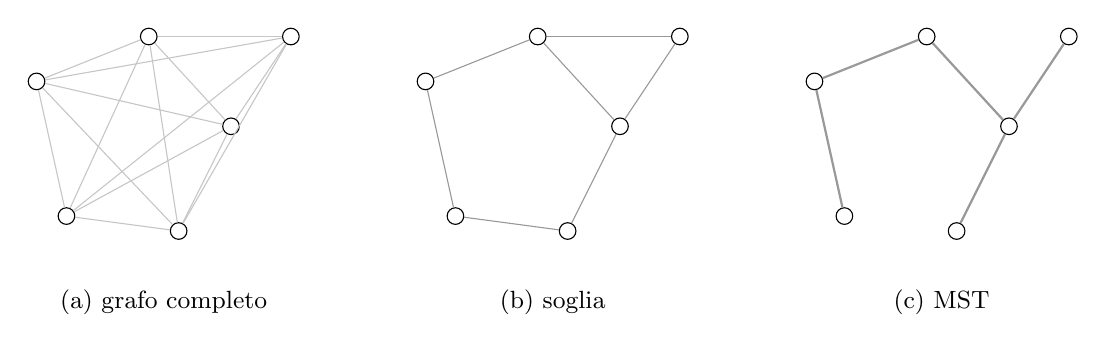
\begin{tikzpicture}[scale=0.95, every node/.style={font=\small},
    nd/.style={circle, draw, fill=white, inner sep=0pt, minimum size=6pt}]
\foreach \s/\dx/\lab in {0/0/{(a) grafo completo}, 1/5.2/{(b) soglia}, 2/10.4/{(c) MST}} {
    \begin{scope}[xshift=\dx cm]
        \node[nd] (n1\s) at (0.0,2.4) {};
        \node[nd] (n2\s) at (1.5,3.0) {};
        \node[nd] (n3\s) at (2.6,1.8) {};
        \node[nd] (n4\s) at (1.9,0.4) {};
        \node[nd] (n5\s) at (0.4,0.6) {};
        \node[nd] (n6\s) at (3.4,3.0) {};
        \node at (1.7,-0.55) {\lab};
    \end{scope}
}
% (a) completo
\foreach \a/\b in {1/2,1/3,1/4,1/5,1/6,2/3,2/4,2/5,2/6,3/4,3/5,3/6,4/5,4/6,5/6} {
    \draw[gray!45] (n\a0)--(n\b0);
}
% (b) soglia
\foreach \a/\b in {1/2,1/5,2/3,2/6,3/4,3/6,4/5} {
    \draw[gray!80] (n\a1)--(n\b1);
}
% (c) MST
\foreach \a/\b in {1/2,1/5,2/3,3/4,3/6} {
    \draw[gray!80, thick] (n\a2)--(n\b2);
}
\end{tikzpicture}
\caption[Strategie di filtraggio del grafo di correlazione]{Effetto delle strategie di filtraggio sullo stesso insieme di sei nodi: il grafo completo ricavato dalla matrice di correlazione (15 archi), la sua versione filtrata per soglia (7 archi) e l'albero ricoprente minimo (5 archi). Lo schema è illustrativo e non deriva da dati reali: serve solo a rendere visibile il compromesso tra fedeltà alla matrice di partenza e sparsità del substrato su cui opera il message passing.}
\label{fig:graph-filtering}
\end{figure}

\begin{table}[H]
\centering
\caption[Confronto tra le strategie di costruzione del grafo]{Confronto tra le strategie di filtraggio. $N$ è il numero di asset, $\tau$ la soglia di correlazione, $k$ il numero di vicini mantenuti per nodo.}
\label{tab:graph-construction}
\begin{tabular}{@{}lcccc@{}}
\toprule
\textbf{Strategia} & \textbf{Archi} & \textbf{Parametri} & \textbf{Connessione} & \textbf{Substrato GNN} \\
\midrule
Grafo completo & $N(N-1)/2$ & nessuno & garantita   & inadeguato (denso) \\
Thresholding   & variabile   & $\tau$   & non garantita & buono \\
$k$-NN         & $\leq kN$   & $k$      & non garantita & buono \\
MST            & $N-1$       & nessuno  & garantita   & povero (albero) \\
PMFG           & $3(N-2)$    & nessuno  & garantita   & buono \\
\bottomrule
\end{tabular}
\end{table}

La \Cref{fig:graph-filtering} illustra l'effetto delle prime tre strategie su un esempio schematico, e la \Cref{tab:graph-construction} ne riassume le proprietà. Nessuna è dominante: thresholding e $k$-NN sono le più adatte a fornire un substrato di message passing, MST e PMFG le più informative dal punto di vista della struttura del mercato. Poiché le due questioni di ricerca della \cref{sec:objectives-research-questions} sono di natura diversa — una previsiva, l'altra descrittiva — è ragionevole che non richiedano lo stesso grafo, e il \Cref{ch:literature-review} confermerà questa separazione di fatto.

Rimane un criterio da esplicitare, lasciato in sospeso dal \Cref{ch:from-cnn-to-gnn}: la densità del grafo non va scelta guardando solo alla fedeltà statistica alla matrice di correlazione. Un grafo troppo denso è statisticamente più fedele ma peggiore come substrato di apprendimento, per l'over-smoothing della \cref{sec:known-limitations-gnn}; un grafo troppo rado perde relazioni reali. Il punto di equilibrio è una scelta progettuale da rendere esplicita.

\section{Grafi dinamici e la questione temporale}
\label{sec:dynamic-graphs-temporal-question}

Finora il grafo è stato trattato come un oggetto fisso, ma la \cref{sec:correlation-dependence-pitfalls} ne ha già prodotto una sequenza: a ogni scorrimento della finestra si ottiene una nuova matrice $C_t$, quindi un nuovo $W_t$, un nuovo Laplaciano $L_t$ e una nuova base di autovettori $U_t$. Il dato di partenza non è un grafo, ma una successione $\{G_t\}_{t}$ di grafi sugli stessi nodi. La questione di ricerca della \cref{sec:objectives-research-questions}, relativa all'evoluzione del mercato nel tempo, vive interamente in questo oggetto.

È cruciale tenere conto del fatto che $U_t$ cambi. I filtri della Spectral CNN sono parametri definiti \emph{rispetto a una specifica base di autovettori}: se la base cambia a ogni finestra, i parametri appresi su $G_t$ non hanno alcun significato su $G_{t+1}$, e l'architettura è semplicemente inapplicabile. La GCN non ha questo problema, perché i suoi parametri $W^{(l)}$ agiscono sullo spazio delle feature e mai sui nodi: la struttura influisce sul calcolo solo attraverso $\hat A$, che si ricalcola a costo trascurabile. Le semplificazioni della \cref{sec:gcn-kipf-welling}, nate per ridurre parametri e costo, sono quindi ciò che rende il modello utilizzabile su un grafo che cambia dinamicamente — un requisito che, nel contesto delle cripto, è fondamentale.

Esistono tre approcci distinti per sfruttare la sequenza.

\subsection{Snapshot indipendenti}
Si applica il modello a ciascun $G_t$ separatamente, trattando le finestre come esempi non correlati. È la scelta più semplice e la più facile da valutare correttamente, ma ignora del tutto che $G_t$ e $G_{t+1}$ condividono quasi tutte le osservazioni e sono quindi fortemente simili: la continuità temporale della struttura, che è precisamente ciò che si vorrebbe studiare, non è adeguatamente considerata.

\subsection{GNN più modulo ricorrente}
Si separano le due dimensioni: una GCN aggrega sui vicini a ogni istante, mentre una rete ricorrente — tipicamente una LSTM — propaga lo stato nel tempo. L'architettura di riferimento è la Graph Convolutional Recurrent Network~\cite{seo2018gcrn}, che sostituisce i prodotti matriciali interni alla cella ricorrente con convoluzioni su grafo. Il modello resta leggibile — si conosce il ruolo di ogni componente — ed è il compromesso più frequente nei lavori applicati.

\subsection{Architetture spazio-temporali integrate}
La ricorrenza è costosa da addestrare e mal parallelizzabile. La \emph{Spatio-Temporal Graph Convolutional Network} (STGCN)~\cite{yu2018stgcn} la sostituisce alternando blocchi di convoluzione su grafo e convoluzioni monodimensionali lungo l'asse temporale, ottenendo un modello interamente convoluzionale e più veloce. La \emph{Diffusion Convolutional Recurrent Neural Network} (DCRNN)~\cite{li2018dcrnn} modella invece la propagazione spaziale come un processo di diffusione su grafo orientato, con un'architettura encoder-decoder per l'orizzonte previsivo. Entrambe nascono per la previsione del traffico stradale, un dominio con una struttura formale analoga a quella di questa tesi — serie temporali su nodi legati da una rete — ma con una differenza sostanziale: nel primo caso il grafo è la rete stradale, fisicamente data e stabile; nel secondo il grafo è stimato dagli stessi dati che si vogliono prevedere.

Due questioni di merito restano aperte. La prima è che il grafo, essendo stimato su una finestra passata, incorpora già informazione sul passato: la struttura è quindi una statistica delle stesse serie che sta prevedendo. A patto che la finestra si chiuda prima dell'istante da prevedere, questo non è di per sé un errore, ma rende meno netta l'interpretazione del contributo della struttura rispetto a quello delle feature. La seconda è la frequenza di aggiornamento del grafo: ricalcolarlo a ogni passo, oppure ogni settimana, o solo a cambi di regime, è un iperparametro che incide fortemente sui risultati.

\section{Il modello VAR come baseline multivariata}
\label{sec:var-baseline}

La prima questione di ricerca della \cref{sec:objectives-research-questions} chiede se modellare esplicitamente le relazioni tra asset porti un vantaggio previsivo. Una domanda di questo tipo ha senso solo rispetto a un termine di paragone, e il termine di paragone naturale è il modello che usa le stesse informazioni senza alcuna struttura a priori: il vettore autoregressivo (VAR) già introdotto nella \cref{sec:limits-univariate-models}.

Raccogliendo i rendimenti degli $N$ asset all'istante $t$ nel vettore $y_t\in\mathbb{R}^N$, il VAR di ordine $p$ si scrive
\begin{equation}
\label{eq:var}
y_t = c + \sum_{i=1}^{p} A_i\,y_{t-i} + \varepsilon_t,
\end{equation}
con $c\in\mathbb{R}^N$ un termine costante, $A_i\in\mathbb{R}^{N\times N}$ le matrici dei coefficienti ed $\varepsilon_t$ un vettore di errori a media nulla e incorrelati nel tempo~\cite{lutkepohl2005new}. Ogni componente di $y_t$ è quindi funzione lineare dei propri $p$ ritardi \emph{e} di quelli di tutti gli altri asset: il modello cattura la dipendenza reciproca senza che le si debba imporre alcuna forma. L'ordine $p$ si sceglie con criteri di informazione — tipicamente AIC o BIC — che bilanciano l'aderenza ai dati con una penalizzazione crescente nel numero di parametri; la stima si riduce poi a $N$ regressioni ai minimi quadrati indipendenti, una per equazione.

Il limite è nel conteggio dei parametri, già anticipato nella \cref{sec:limits-univariate-models} e qui quantificabile: le matrici $A_i$ contengono $N^2p$ coefficienti, cui si aggiungono gli $N$ di $c$. Con $N=50$ asset e $p=5$ ritardi si tratta di $12\,550$ parametri, da stimare su serie che raramente offrono più di qualche migliaio di osservazioni utili — e che, per i fatti stilizzati della \cref{sec:financial-time-series-returns}, contengono un segnale debole. Il modello finisce per adattarsi al rumore. Le versioni regolarizzate~\cite{basu2015regularized} attenuano il problema imponendo sparsità sui coefficienti, cioè assumendo che la maggior parte delle relazioni tra asset sia assente — la stessa assunzione di sparsità che ha motivato il filtraggio del grafo nella \cref{sec:correlation-matrix-to-graph}.

\subsection{La struttura a grafo del VAR}

La matrice $A_i$ dell'equazione~\eqref{eq:var} è una matrice di adiacenza pesata: l'entrata $(A_i)_{jk}$ misura quanto il rendimento dell'asset $k$ a $i$ passi di distanza contribuisce a quello dell'asset $j$. Se il coefficiente è nullo per ogni ritardo, l'asset $k$ non aiuta a prevedere $j$ — che è precisamente la definizione di assenza di causalità di Granger~\cite{granger1969investigating}\footnote{Il termine \enquote{causalità} va inteso in senso puramente previsivo: $k$ causa $j$ secondo Granger se il passato di $k$ migliora la previsione di $j$ rispetto a quella basata sul solo passato di $j$. Non si tratta di causalità in senso fisico, e la relazione può benissimo riflettere un fattore comune non osservato.}. Il VAR costruisce dunque un grafo dai dati, e la sua struttura è quella dei test di causalità di Granger tra tutte le coppie di asset.

La differenza rispetto all'approccio di questa tesi riguarda dunque la \emph{collocazione della conoscenza sulla struttura}. Il VAR stima ogni relazione dai dati, ottenendo un grafo orientato, potenzialmente denso e costoso in parametri. La GCN riceve invece un grafo esplicito, non orientato e sparso, costruito con i criteri della \cref{sec:correlation-matrix-to-graph}, e usa i parametri risparmiati per apprendere una trasformazione non lineare delle feature. Si tratta di uno scambio tra distorsione e varianza applicato alla struttura: il VAR ha meno distorsione e più varianza, mentre per la GCN vale la relazione opposta. Il confronto tra VAR e GCN è quindi informativo su una questione precisa: se il grafo di correlazione, nonostante i compromessi che la sua costruzione richiede, sia un'ipotesi a priori abbastanza buona da giustificare il vincolo che impone. Il \Cref{ch:literature-review} mostrerà che solitamente ci si limita a confrontare le prestazioni predittive senza mettere in discussione il grafo di correlazione come ipotesi.
